\documentclass{article}\usepackage[]{graphicx}\usepackage[]{color}
%% maxwidth is the original width if it is less than linewidth
%% otherwise use linewidth (to make sure the graphics do not exceed the margin)
\makeatletter
\def\maxwidth{ %
  \ifdim\Gin@nat@width>\linewidth
    \linewidth
  \else
    \Gin@nat@width
  \fi
}
\makeatother

\definecolor{fgcolor}{rgb}{0.345, 0.345, 0.345}
\newcommand{\hlnum}[1]{\textcolor[rgb]{0.686,0.059,0.569}{#1}}%
\newcommand{\hlstr}[1]{\textcolor[rgb]{0.192,0.494,0.8}{#1}}%
\newcommand{\hlcom}[1]{\textcolor[rgb]{0.678,0.584,0.686}{\textit{#1}}}%
\newcommand{\hlopt}[1]{\textcolor[rgb]{0,0,0}{#1}}%
\newcommand{\hlstd}[1]{\textcolor[rgb]{0.345,0.345,0.345}{#1}}%
\newcommand{\hlkwa}[1]{\textcolor[rgb]{0.161,0.373,0.58}{\textbf{#1}}}%
\newcommand{\hlkwb}[1]{\textcolor[rgb]{0.69,0.353,0.396}{#1}}%
\newcommand{\hlkwc}[1]{\textcolor[rgb]{0.333,0.667,0.333}{#1}}%
\newcommand{\hlkwd}[1]{\textcolor[rgb]{0.737,0.353,0.396}{\textbf{#1}}}%

\usepackage{framed}
\makeatletter
\newenvironment{kframe}{%
 \def\at@end@of@kframe{}%
 \ifinner\ifhmode%
  \def\at@end@of@kframe{\end{minipage}}%
  \begin{minipage}{\columnwidth}%
 \fi\fi%
 \def\FrameCommand##1{\hskip\@totalleftmargin \hskip-\fboxsep
 \colorbox{shadecolor}{##1}\hskip-\fboxsep
     % There is no \\@totalrightmargin, so:
     \hskip-\linewidth \hskip-\@totalleftmargin \hskip\columnwidth}%
 \MakeFramed {\advance\hsize-\width
   \@totalleftmargin\z@ \linewidth\hsize
   \@setminipage}}%
 {\par\unskip\endMakeFramed%
 \at@end@of@kframe}
\makeatother

\definecolor{shadecolor}{rgb}{.97, .97, .97}
\definecolor{messagecolor}{rgb}{0, 0, 0}
\definecolor{warningcolor}{rgb}{1, 0, 1}
\definecolor{errorcolor}{rgb}{1, 0, 0}
\newenvironment{knitrout}{}{} % an empty environment to be redefined in TeX

\usepackage{alltt}

\title{Santa Ana Sucker Habitat Evaluation}
\author{C. Flynn, E. Harris-Tyrrell, O. Howie, L. Israel, S. Janessn, \\N. Larson, F. Lyles, W. Norena, V. Sanchez-Jimenez, A. Vacas, D. Wagner,\\ ed. Marc Los Huertos}
\IfFileExists{upquote.sty}{\usepackage{upquote}}{}
\begin{document}

\maketitle

\newpage
\tableofcontents
\newpage

\section{Introduction}


\subsection{Problem Statement}



\subsection{Background (Literature Review)}

 
\subsection{Background Research w/Citations} 

Albertson, L.K., Koenig, L.E., Lewis, B.L., Zeug, S.C., Harrison, L.R., \& Cardinale, B.J. (2012). How Does Restored Habitat for Chinook Salmon (Oncorhynchus Tshawytscha) in the Merced River in California Compare with other Chinook Streams? River Research and Applications, 29(4), 469-482). doi: 10.1002/rra.1604

By looking at Chinook salmon in the Merced river, restoration projects seemed to be failing to prevent the Chinook population from falling. The installation of gravel augmentation in a reconfigured channel seemed to have little impact on the salmon, suggesting that other factors were catalyzing the fall of the species. By comparing the restored portion with other portions of the Merced river, food web characteristics and flow discharge seemed to produce the same results on the various life stages of the salmon. However, higher temperatures, less woody debris, and minimal riparian cover seemed to limit populations in the restored portions. Restoration efforts are then presented with an added challenge of ensuring that every aspect of the ecosystem is beneficial to the species, which demands more work toward temperature regulation and attempts to restore the river bank. To see how the Santa Ana sucker would react to similar conservation efforts would be interesting in discussions in attempting to determine solutions. 

Coulter, D. P., Höök, T. O., Mahapatra, C. T., Guffey, S. C., \& Sepúlveda, M. S. (2015). Fluctuating Water Temperatures Affect Development, Physiological Responses and Cause Sex Reversal in Fathead Minnows. Environmental Science \& Technology, 49(3), 1921-1928. doi:10.1021/es5057159

Human activities can increase water temperature. Water-based organisms are sensitive to temperature change, especially young fish due to limited mobility. This paper explained how young Flathead Minnows exposed to warmer temperatures underwent a nondirectional sex reversal. This paper shows us how temperature can greatly affect fish and stress them out. Clearly, water temperature drastically affects fish, not necessarily in a positive way, and therefore, we should see if there is a correlation between stream temperature and where the Santa Ana Sucker chooses to live.

Los Huertos, Marc. (2016). Thermal Properties of Water. Environmental Science of Aquatic Systems. 297-308.

Temperature varies greatly in its impact on fish depending upon the conditions affecting the lake or river. Heat, temperature, thermal energy, and heat capacity all slightly change how heat is measured in an ecosystem. Water in general has a high heat capacity, which indicates its high specific heat. These aquatic systems therefore often retain their heat and are less susceptible to increase/decrease in temperature. Inflows/mixing can have an effect on water temperature but it is often hard to detect due to thermal stratification mixing, seasonal change in temperature profile depth, and small volume inflow in terms of fraction of the lake volume. This chapter sheds light that variations in temperature trigger chemicals dissolving/remaining, tend to raise/lower a fish’s body temperature to the same degree, etc. Temperature impacts many other features of water quality, which will be important to keep in mind going forward with the project.

Sadler, K. (1980). Effect of the warm water discharge from a power station on fish populations in the river Trent. Journal Of Applied Ecology, 17(2):349-357.

A power station discharged water that was on average 7 degrees Celsius above normal in the River Trent. This meant that in affected areas, the winter migration was delayed from Sep/Oct to Dec/Jan, while in unaffected areas, migration continued at normal times. Also, below the power station, fish preferred to live further downstream, in terms of diversity and population density. This tells us that fish are able to change their living patterns based on water temperature, and shows that fish were noticeably affected by the temperature change. 

U.S. Fish \& Wildlife Service. 2012. Recovery Outline for Santa Ana sucker. Sacramento, California. 38 pp.

This report discusses Santa Ana Suckers and possible recovery plans. In order to do so, it clearly outlines Sucker habitat preferences, behavior, and threats. We used this source to determine preferred temperature for the Santa Ana Sucker and in general to inform ourselves more about the fish. Little research has been done on specific threats to the Santa Ana Sucker, but the document did point out possible threats arising from hydrological modification and urban development in general. Sophie and I thought that potentially water coming out of a treatment plant could be a threat under hydrological modification or urban development, so that will be what our research focuses on.

\subsection{Objectives}
Our goal with this experiment was to find out whether or not temperature was affecting the population and/or livelihood of the Santa Ana Sucker in the Santa Ana River.

\subsection{Materials and Equipment}

4 HOBO Tidbit Water Temperature Data Logger,
1 Optic USB U-4 Base Station,
1 Coupler,
4 Green Garden stakes,
Red flags,
Yellow marking tape,
Free HOBOware software,
Transportation to and from the river,
Ice Bath

\subsection{Methods}

We will obtain four HOBO Tidbit water temperature Data Loggers to set up at the Rialto Channel at Agua Mansa (site 4), another at the point where the other discharge site meets the river (site 2), another just above that site (site 3), and a fourth in the pool where Suckers have previously been observed (site 1). Before going to the river, we programmed the loggers via our base station and the HOBOware software to collect water temperature data every 15 minutes. In order to start the data process, we put each logger into the coupler and pushed the level til the light was flashing. We then put them in the river by looping a garden stake through one, sticking it into the substrate, and securing it with rocks. We then put yellow marking tape on plants nearby and red flags along the bank to show where we left the main path. We repeated this for each site, making sure the loggers were secure and fairly hidden. After seven nights (for site 3) and eleven nights (for the other sites), we returned to the river and collected the loggers. In the lab, using the software, we loaded our data and transferred it to RStudio. Later, to calibrate the loggers, we put them in an ice bath for 6 minutes to ensure that the temperature settled around zero and each logger was measuring to the same temperature with the same accuracy.

\subsection{Site Descrition}

We evaluated the Santa Ana River between... near Colton, California (Figure \ref{SAR_Image}). 

\begin{figure}
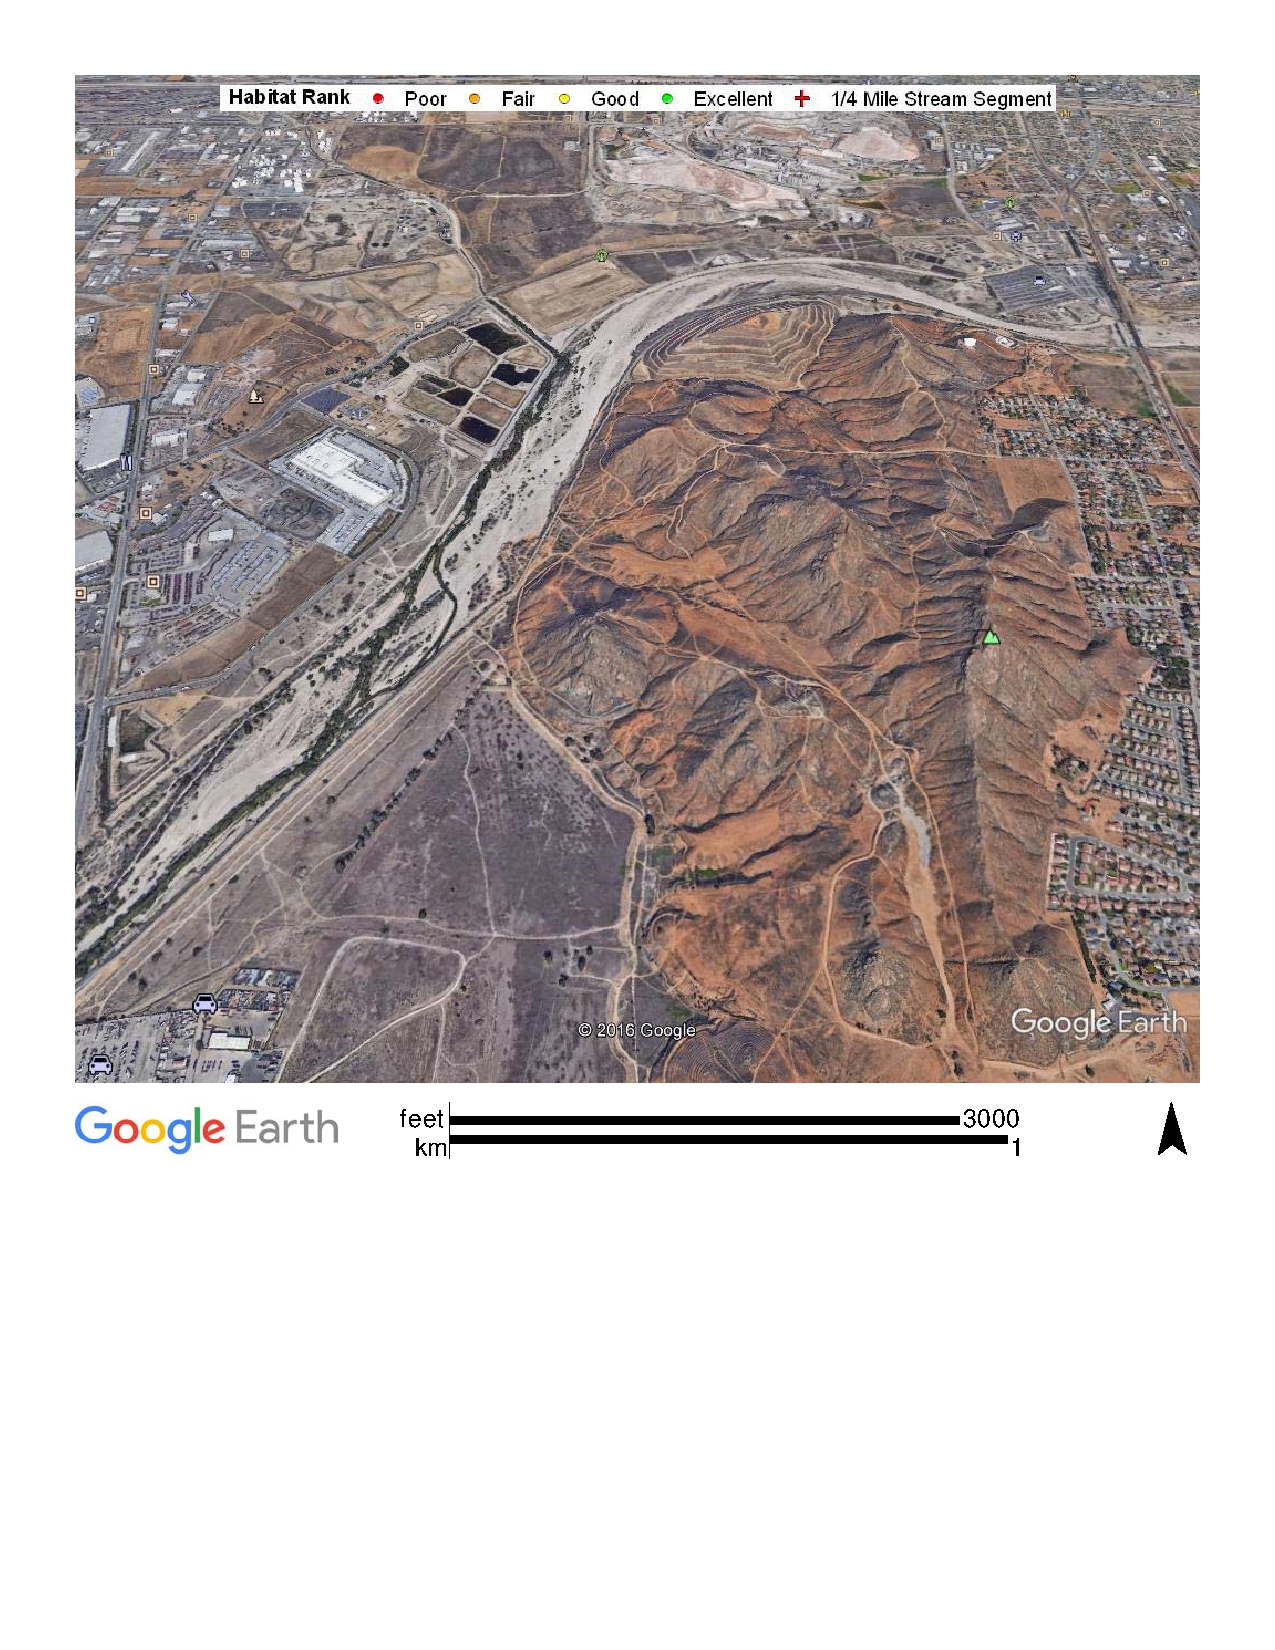
\includegraphics[width=1.00\textwidth]{Figures/SantaAna_SatelliteImage}
\caption{Google Earth --Example of a map. What's wrong with this image?}
\label{SAR_Image}
\end{figure}

\subsection{Field Methods}

\subsection{Laboratory Methods}

\subsection{Statistical Methods}

\section{Results}

The tempeature data suggests... (Figure \ref{Temp}).

\begin{figure}
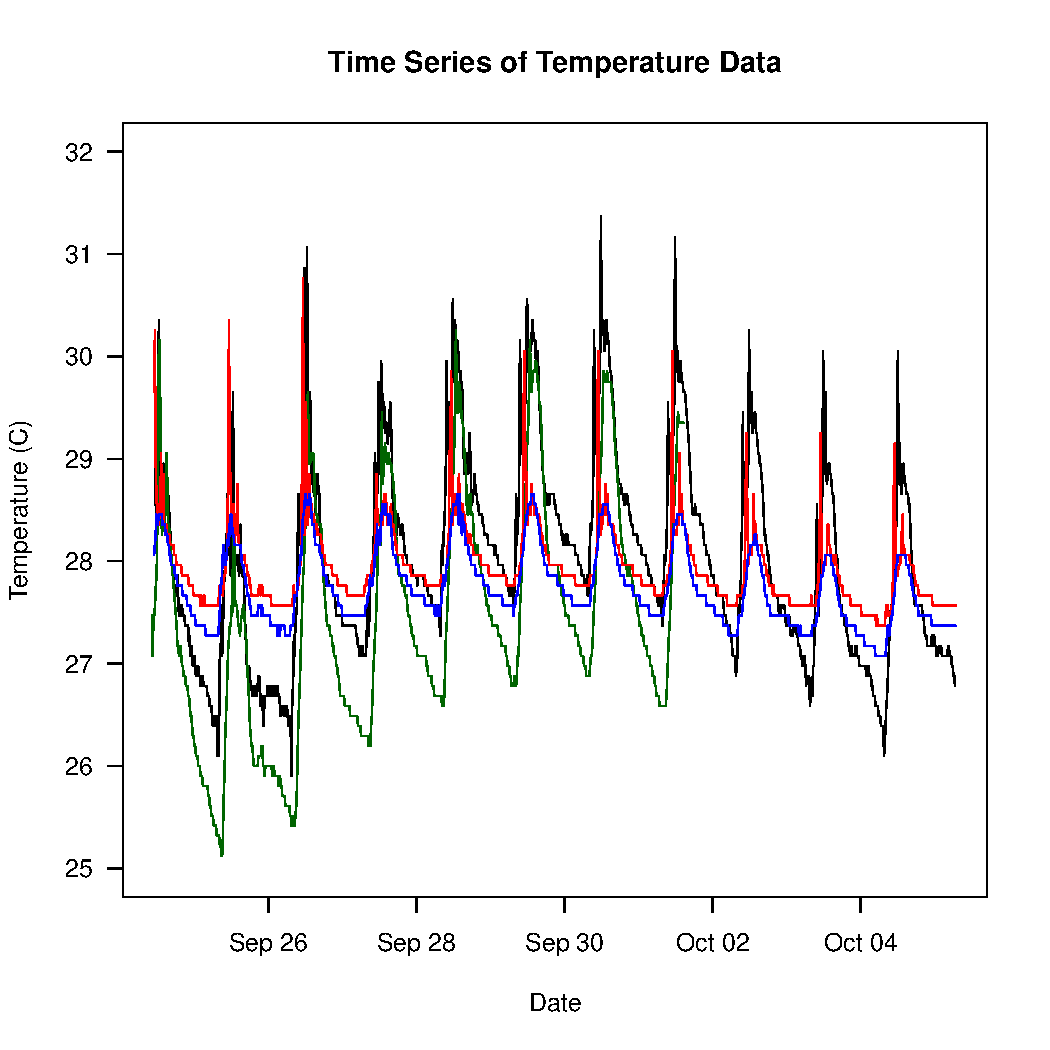
\includegraphics{Figures/Temp}
\caption{Temperature time...}
\label{Temp}
\end{figure}

\section{Discussion}


\section{Conclusion and Recommendations}


\end{document}
